\documentclass[10pt,a4paper]{article}
\usepackage[utf8]{inputenc}
\usepackage[spanish]{babel}
\usepackage{amsmath}
\usepackage{amsfonts}
\usepackage{amssymb}
\usepackage{amsthm}
\usepackage{graphicx}
\usepackage{subcaption}
\usepackage[]{algorithm2e}
\usepackage{float}
\author{Carlos Manuel Rodríguez Martínez}
\title{Optimización de Redes Bayesianas por medio de un Algoritmo Genético}

\newtheorem{definition1}{Definición}
\newtheorem{teorema1}{Teorema}
\newtheorem{corolario}{Corolario}[teorema1]

\begin{document}
\maketitle

\section{Fórmula de Robinson}
En 1977, Robinson \cite{Robinson1977} publica una fórmula que devuelve la cantidad de grafos DAG dado un número $n$ de vértices,
\[
	f(n) = \sum_{i=1}^n (-1)^{i+1} \binom{n}{i} 2^{i(n-i)} f(n-i).
\]

Se realizó una implementación de la fórmula utilizando el lenguaje Wolfram.
\begin{figure}[h!]
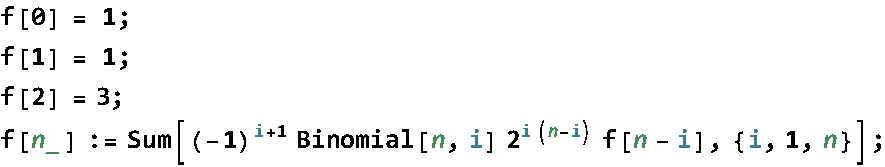
\includegraphics[scale=0.6]{img/formula}
\end{figure}

Al evaluar la fórmula en un invervalo del $[1,9]$ se observa el crecimiento (exponencial?) de la función.
\begin{figure}[h!]
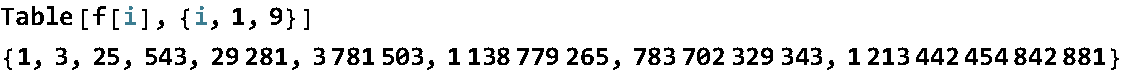
\includegraphics[scale=0.6]{img/formulaEval}
\end{figure}

Esta secuencia se encuentra en el OEIS como A003024 \cite{oeis}. En el 2003, Eric Weisstein encontró numéricamente que el número de matrices (0,1) de tamaño $n \times n$ cuyos eigenvalores son reales y positivos coincide con la secuencia A003024 \cite{weisstein}.

\section{Algoritmo generador de DAG}
El objetivo a resolver en este problema es generar un algoritmo que enliste todos los posibles grafos acíclicos dirigidos (o DAG por sus siglas en inglés). Un DAG es un grafo dirigido que no posee ciclos, esto es, dado un vértice $v$ no existe ninguna secuencia de transiciones que nos regrese al mismo vértice $v$.

\begin{figure}[h!]
\centering
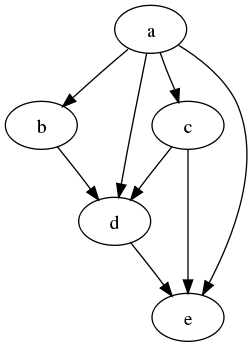
\includegraphics[scale=0.4]{img/DAG}
\caption{Ejemplo de DAG. Nótese que no existe ninguna secuencia de transiciones que comenzando desde un estado (por ejemplo el $b$), nos regrese al mismo.}
\end{figure}


\subsection{Matriz de adyacencia}
Un grafo está definido formalmente por una serie de vértices relacionados por nodos que especifican la relación entre los vértices. Sea $V$ el conjunto de vértices de un grafo, se puede construir una representación matricial del grafo a partir de una matriz cuadrada $A$ de tamaño $|V| \times |V|$ tal que sus elementos $A_{ij}$ sean $1$ cuando exista un nodo entre el $V_i$ y $V_j$, y $0$ cuando no exista.

\subsubsection*{Ejemplo}
En la figura \ref{fig:grafos} se muestra un ejemplo de grafo DAG con su respectiva representación en forma de matriz de adyacencia. Nótese que toda matriz de adyacencia estrictamente triangular superior
\[
A = \begin{cases} 
      A_{ij} & 1 < j < i \\
     0 & \text{en caso contrario} \\
    \end{cases}
\]
representa un DAG.

\begin{figure}[h!]
		\begin{subfigure}{.5\textwidth}
			\centering
			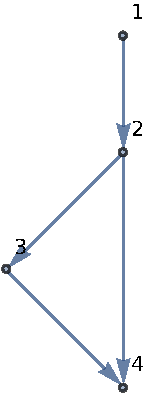
\includegraphics[scale=0.45]{img/graph}
			\caption{Grafo DAG, definido por los vértices entre los nodos.}
		\end{subfigure}%
		\begin{subfigure}{.5\textwidth}
			\centering
			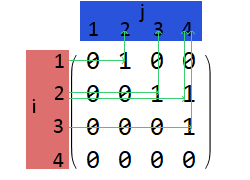
\includegraphics[scale=0.45]{img/ady_matrix}
			\caption{Representación matricial del mismo grafo.}
		\end{subfigure}%
		\caption{Ejemplo de DAG y sus representaciones.}
		\label{fig:grafos}
\end{figure}

\subsection{Representaciones equivalentes de la matriz de adyacencia de un DAG}
Debido a la forma en la que está construida la matriz de adyacencia es posible renombrar los índices de los vértices sin alterar la estructura del grafo. En la figura \ref{fig:th} se muestra el mismo grafo que en la figura \ref{fig:grafos} con la única diferencia de que se ha invertido la posición de los índices 1 y 2 en $j$. Esto no afecta a la estructura del grafo ya que la posición de los índices es sólo una convención. Se dice que dos digrafos acíclicos son isomorfos si existe un mapeo uno a uno entre ambos que preserva las relaciones de adyacencia.

\begin{figure}[h!]
\centering
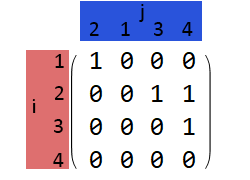
\includegraphics[scale=0.4]{img/t12v_matriz}
\caption{El mismo DAG de la figura \ref{fig:grafos} con los índices 1 y 2 en $j$ invertidos.}
\label{fig:th}
\end{figure}

La posibilidad de invertir índices sin afectar la estructura del grafo nos permite definir un conjunto de transformaciones que sobre la matriz de adyacencia que representan el mismo grafo.

\begin{definition1}
Sea $A$ una matriz que representa a un grafo, se define la función de inversión de índices $\alpha$, $\beta$ vertical como
\[
	T_{\alpha \beta V}(A) = 
	\begin{cases} 
      A_{i \beta} & j = \alpha \\
      A_{i \alpha} & j =  \beta \\
      A_{ij} & j \neq \alpha, \beta
    \end{cases}
\]
y la función de inversión de índices $\alpha$, $\beta$ horizontal como
\[
	T_{\alpha \beta H}(A) = 
	\begin{cases} 
      A_{\beta j} & i = \alpha \\
      A_{\alpha i} & i =  \beta \\
      A_{ij} & i \neq \alpha, \beta
    \end{cases}
\]
\end{definition1}
Nótese que todas las transformaciones $T$ cumplen la propiedad de linealidad
\begin{align*}
	T(A) + T(B) &= T(A+B), \\
	T(cA) &= c T(A).
\end{align*}

\subsubsection*{Ejemplo}
Si
\[
	A = \begin{pmatrix}
		a & b & c \\
		d & e & f \\
		g & h & i
	\end{pmatrix},
\]
entonces
\[
	T_{12H}(A) = \begin{pmatrix}
		b & a & c \\
		e & d & f \\
		h & g & i
	\end{pmatrix},\quad
	T_{12V}(A) = \begin{pmatrix}
		d & e & f \\
		a & b & c \\
		g & h & i
	\end{pmatrix},
\]

\subsection{Eigenvalores de la matriz de adyacencia}
Supongamos que $A$ representa la matriz de adyacencia de un grafo $G$, esto es, $A = A (G)$. $A$ sólo debe tener ceros en su diagonal, de lo contrario habría ciclos de los vértices consigo mismos. Se define $B = I + A$, la cual tiene también la propiedad de ser una matriz booleana. Si el grafo $G$ es un DAG, entonces siempre debe ser posible obtener una matriz estrictamente triangular superior por medio de una composición de transformaciones $T_{\alpha \beta V}$ y $T_{\alpha \beta H}$. Entonces los eigenvalores $\lambda$ de $B$ están dados por
\[
 \begin{vmatrix}
  1 - \lambda & x & \cdots & y \\
  0 & 1 - \lambda & \cdots & z \\
  \vdots  & \vdots  & \ddots & \vdots  \\
  0 & 0 & \cdots & 1 - \lambda 
 \end{vmatrix} = 0
\]
cuya única solución es $\lambda = 1$.

\begin{teorema1}
Sea $A$ una matriz de adyacencia que representa un grafo $G$, se define la transformación
\[
T_{\alpha \beta} (A) = T_{\alpha \beta H}(T_{\alpha \beta V}(A)) = T_{\alpha \beta V}(T_{\alpha \beta H}(A)),
\]
y la función $\operatorname{det}(A)$ que representa la determinante de $A$. Entonces
$\operatorname{det}(A) = \operatorname{det}(T_{\alpha \beta} (A))$.
\end{teorema1}

\begin{proof}
Cada operación de intercambio de filas o columnas tiene el efecto de invertir el signo de la determinante, esto es
\begin{align*}
	\operatorname{det}\left( T_{\alpha \beta H}(A) \right) &= \sum_{ijk} \epsilon_{ijk} A_{2i} A_{1j} A_{3k} \\
	&= \sum_{ijk} \epsilon_{ijk} A_{1j} A_{2i} A_{3k} \\
	&= - \sum_{jik} \epsilon_{jik} A_{1j} A_{2i} A_{3k} = - \operatorname{det}(A).
\end{align*}
Mediante un procedimiento análogo se puede probar también que
\[
	\operatorname{det}\left( T_{\alpha \beta V}(A) \right) = - \operatorname{det}(A),
\]
por lo tanto
\[
	\operatorname{det}(T_{\alpha \beta} (A)) = \operatorname{det}(A).
\]

\end{proof}
A partir de este resultado y haciendo uso de la propiedad de linealidad de las transformaciones $T$ se obtiene el siguiente corolario.
\begin{corolario}
\label{cor1}
El conjunto de transformaciones $T$ no altera los eigenvalores de la matriz de adyacencia.
\end{corolario}
\begin{proof}
Asumiendo que $T$ representa a cualquier operador del tipo $T_{\alpha \beta}$, $T_{\alpha \beta H}$ o $T_{\alpha \beta V}$, y haciendo uso de la propiedad de linealidad, se tiene que
\[
	\operatorname{eigen}(T(A)) = |T(A) - \lambda I| = |T(A-\lambda I)| = |A-\lambda I| = \operatorname{eigen}(A).
\]
\end{proof}

\subsection{Especificación de algoritmo}
El resultado del corolario \ref{cor1} nos lleva a que si $A$ representa un DAG, entonces los eigenvalores de una matriz de adyacencia de un grafo equivalente deben ser también $\lambda = 1$. Se puede comprobar fácilmente que cualquier DAG tiene una representación equivalente en forma de matriz triangular superior, por ejemplo, el DAG representado por la matriz
\[
	A = \begin{pmatrix}
		0 & 0 & 0 \\
		1 & 0 & 1 \\
		1 & 0 & 0
	\end{pmatrix}
\]
tiene una representación equivalente en forma de matriz triangular superior dada por las transformaciones
\[
	T_{12} \circ T_{13} (A) = T_{13} \circ T_{23} (A) = T_{12} \circ T_{23} (A) = \begin{pmatrix}
		0 & 1 & 1 \\
		0 & 0 & 1 \\
		0 & 0 & 0
	\end{pmatrix},
\]
en consecuencia los eigenvalores de $A+I$ son $\lambda_i (A+I) = 1$.
El algoritmo generador de DAG que se realizó en esta tarea se basará en esta propiedad.

\begin{algorithm}[H]
 \KwData{tamaño grafo n}
 \KwResult{Matrices correspondientes a un DAG }
 Generar todas las matrices de adyacencia posibles a partir de permutaciones de n-tuplas con elementos \{0,1\}\;
 \ForEach{Matriz de adyacencia $A_i = A(G_i)$}{
 Obtener eigenvalores $\lambda_i = \lambda(A_i)$\;
 \eIf{$|\lambda_i| = 1$}{
   $A$ representa un DAG\;
   }{
   $A$ \textbf{no} representa un DAG\;
  }
 }
 \caption{Algoritmo generador de matrices de adyacencia DAG.}
\end{algorithm}

\subsection{Implementación del algoritmo}
El algoritmo se implementó en el lenguaje Wolfram, y se construye como sigue.
Construir matriz a partir de parámetros.
\begin{figure}[H]
\centering
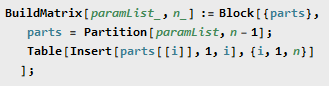
\includegraphics[scale=0.6]{img/codigo1}
\end{figure}

Generar los parámetros como permutaciones de tuplas.

\begin{figure}[H]
\centering
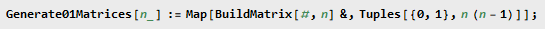
\includegraphics[scale=0.6]{img/codigo2}
\end{figure}

Seleccionar las matrices que corresponden a un DAG.

\begin{figure}[H]
\centering
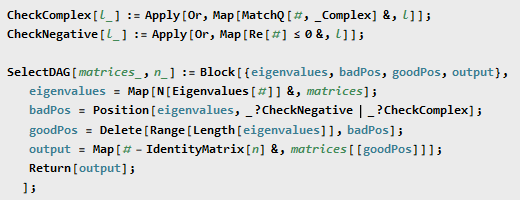
\includegraphics[scale=0.6]{img/codigo3}
\end{figure}

Listar todos los DAG de orden $n$.

\begin{figure}[H]
\centering
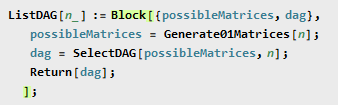
\includegraphics[scale=0.6]{img/codigo4}
\end{figure}


\subsection{Resultados}
En las figuras \ref{fig:resultado1}, \ref{fig:resultado2}, \ref{fig:resultado3} y \ref{fig:resultado4} se muestran los resultados para DAG de orden hasta $n=3$. En la fórmula de Robinson se puede ver que la cantidad de soluciones crece de manera tan rápida que nuestra capacidad de cómputo pronto queda opacada al tratar de listar los DAG para $n>5$.

\begin{figure}[h!]
\centering
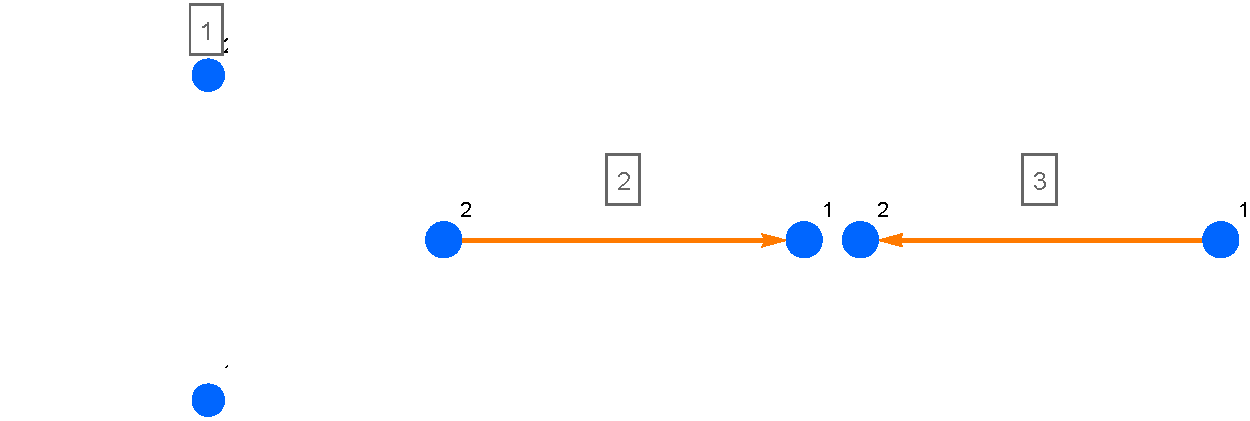
\includegraphics[scale=0.6]{img/grafosDAG2}
\caption{Grafos DAG con $n=2$.}
\label{fig:resultado1}
\end{figure}

\begin{figure}[h!]
\centering
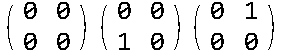
\includegraphics[scale=0.8]{img/matrixDAG2}
\caption{Matrices de adyacencia DAG con $n=2$.}
\label{fig:resultado2}
\end{figure}

\begin{figure}[h!]
\centering
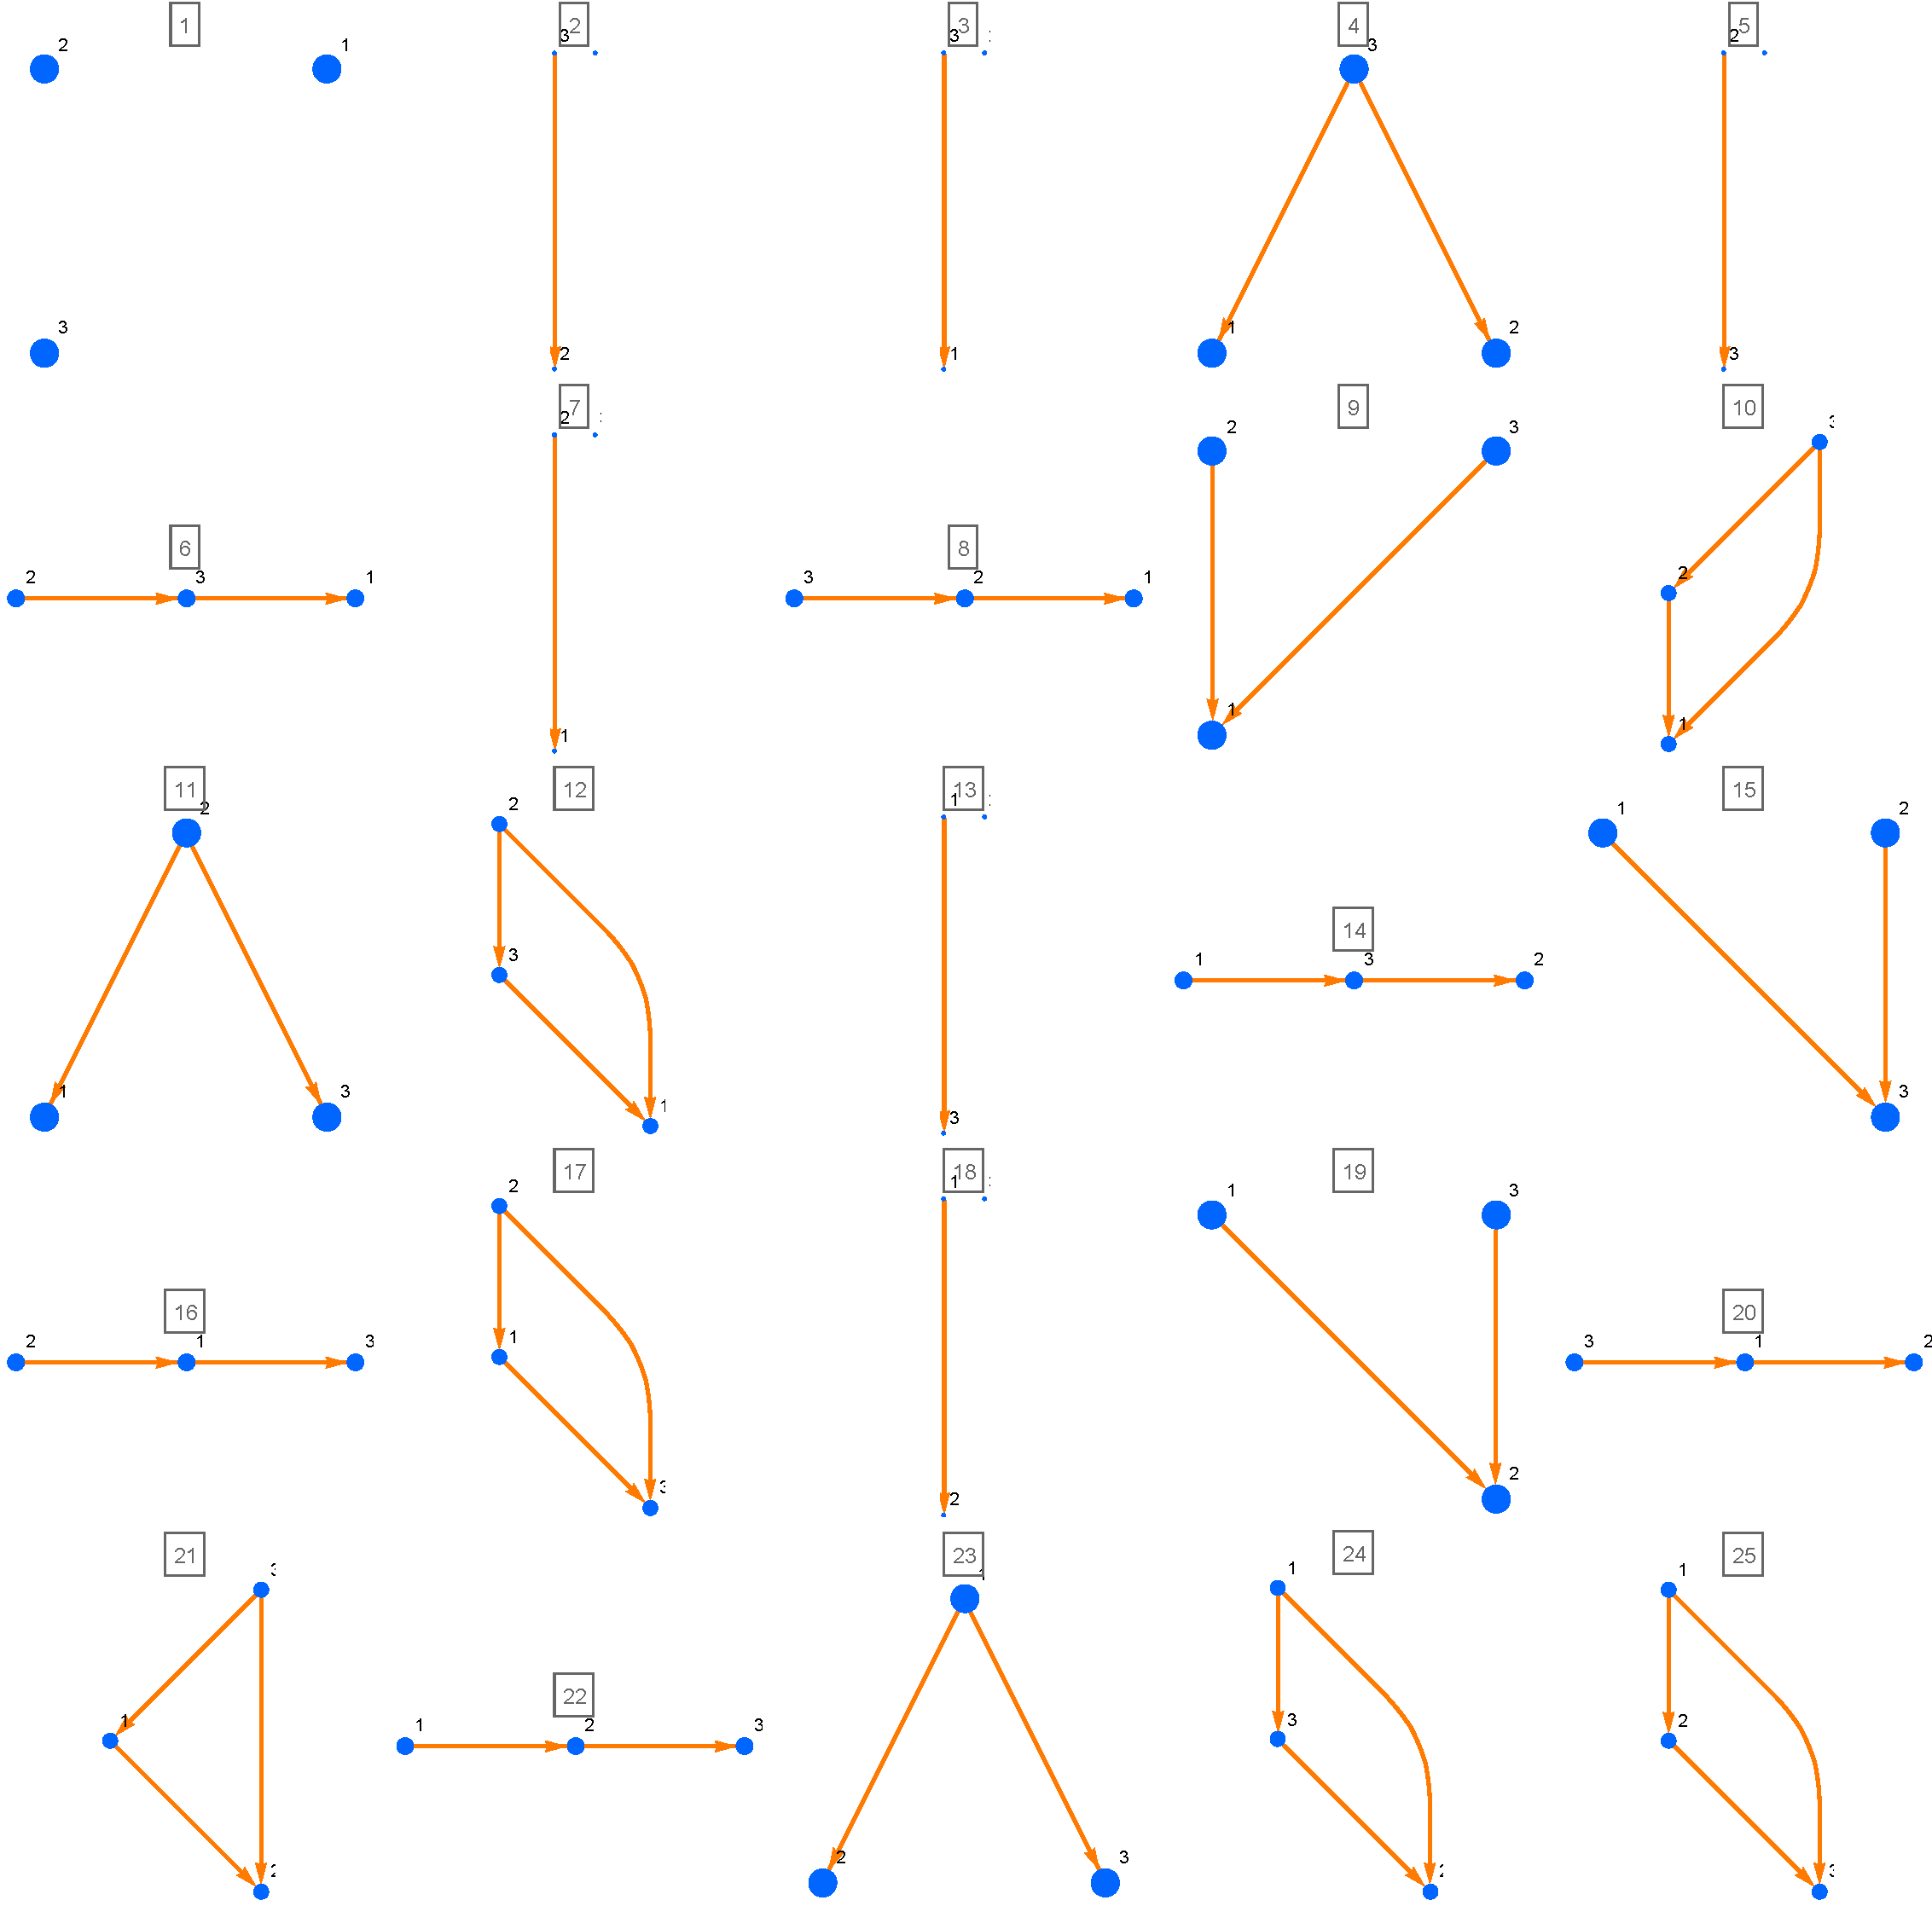
\includegraphics[scale=0.3]{img/grafosDAG3}
\caption{Grafos DAG con $n=3$.}
\label{fig:resultado3}
\end{figure}

\begin{figure}[h!]
\centering
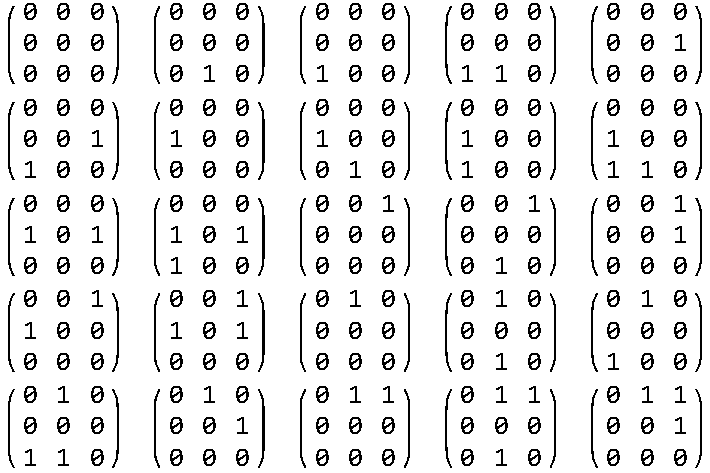
\includegraphics[scale=0.8]{img/matrixDAG3}
\caption{Matrices de adyacencia DAG con $n=3$.}
\label{fig:resultado4}
\end{figure}

\clearpage
\nocite*
\bibliography{Referencias}{}
\bibliographystyle{plain}

\end{document}